\section{Process mining}
\label{sec:process_mining}

We mined the logs generated by the simulation of the collapsed workflow.

We modified the simulation configuration 

\begin{figure}[H]
\centering
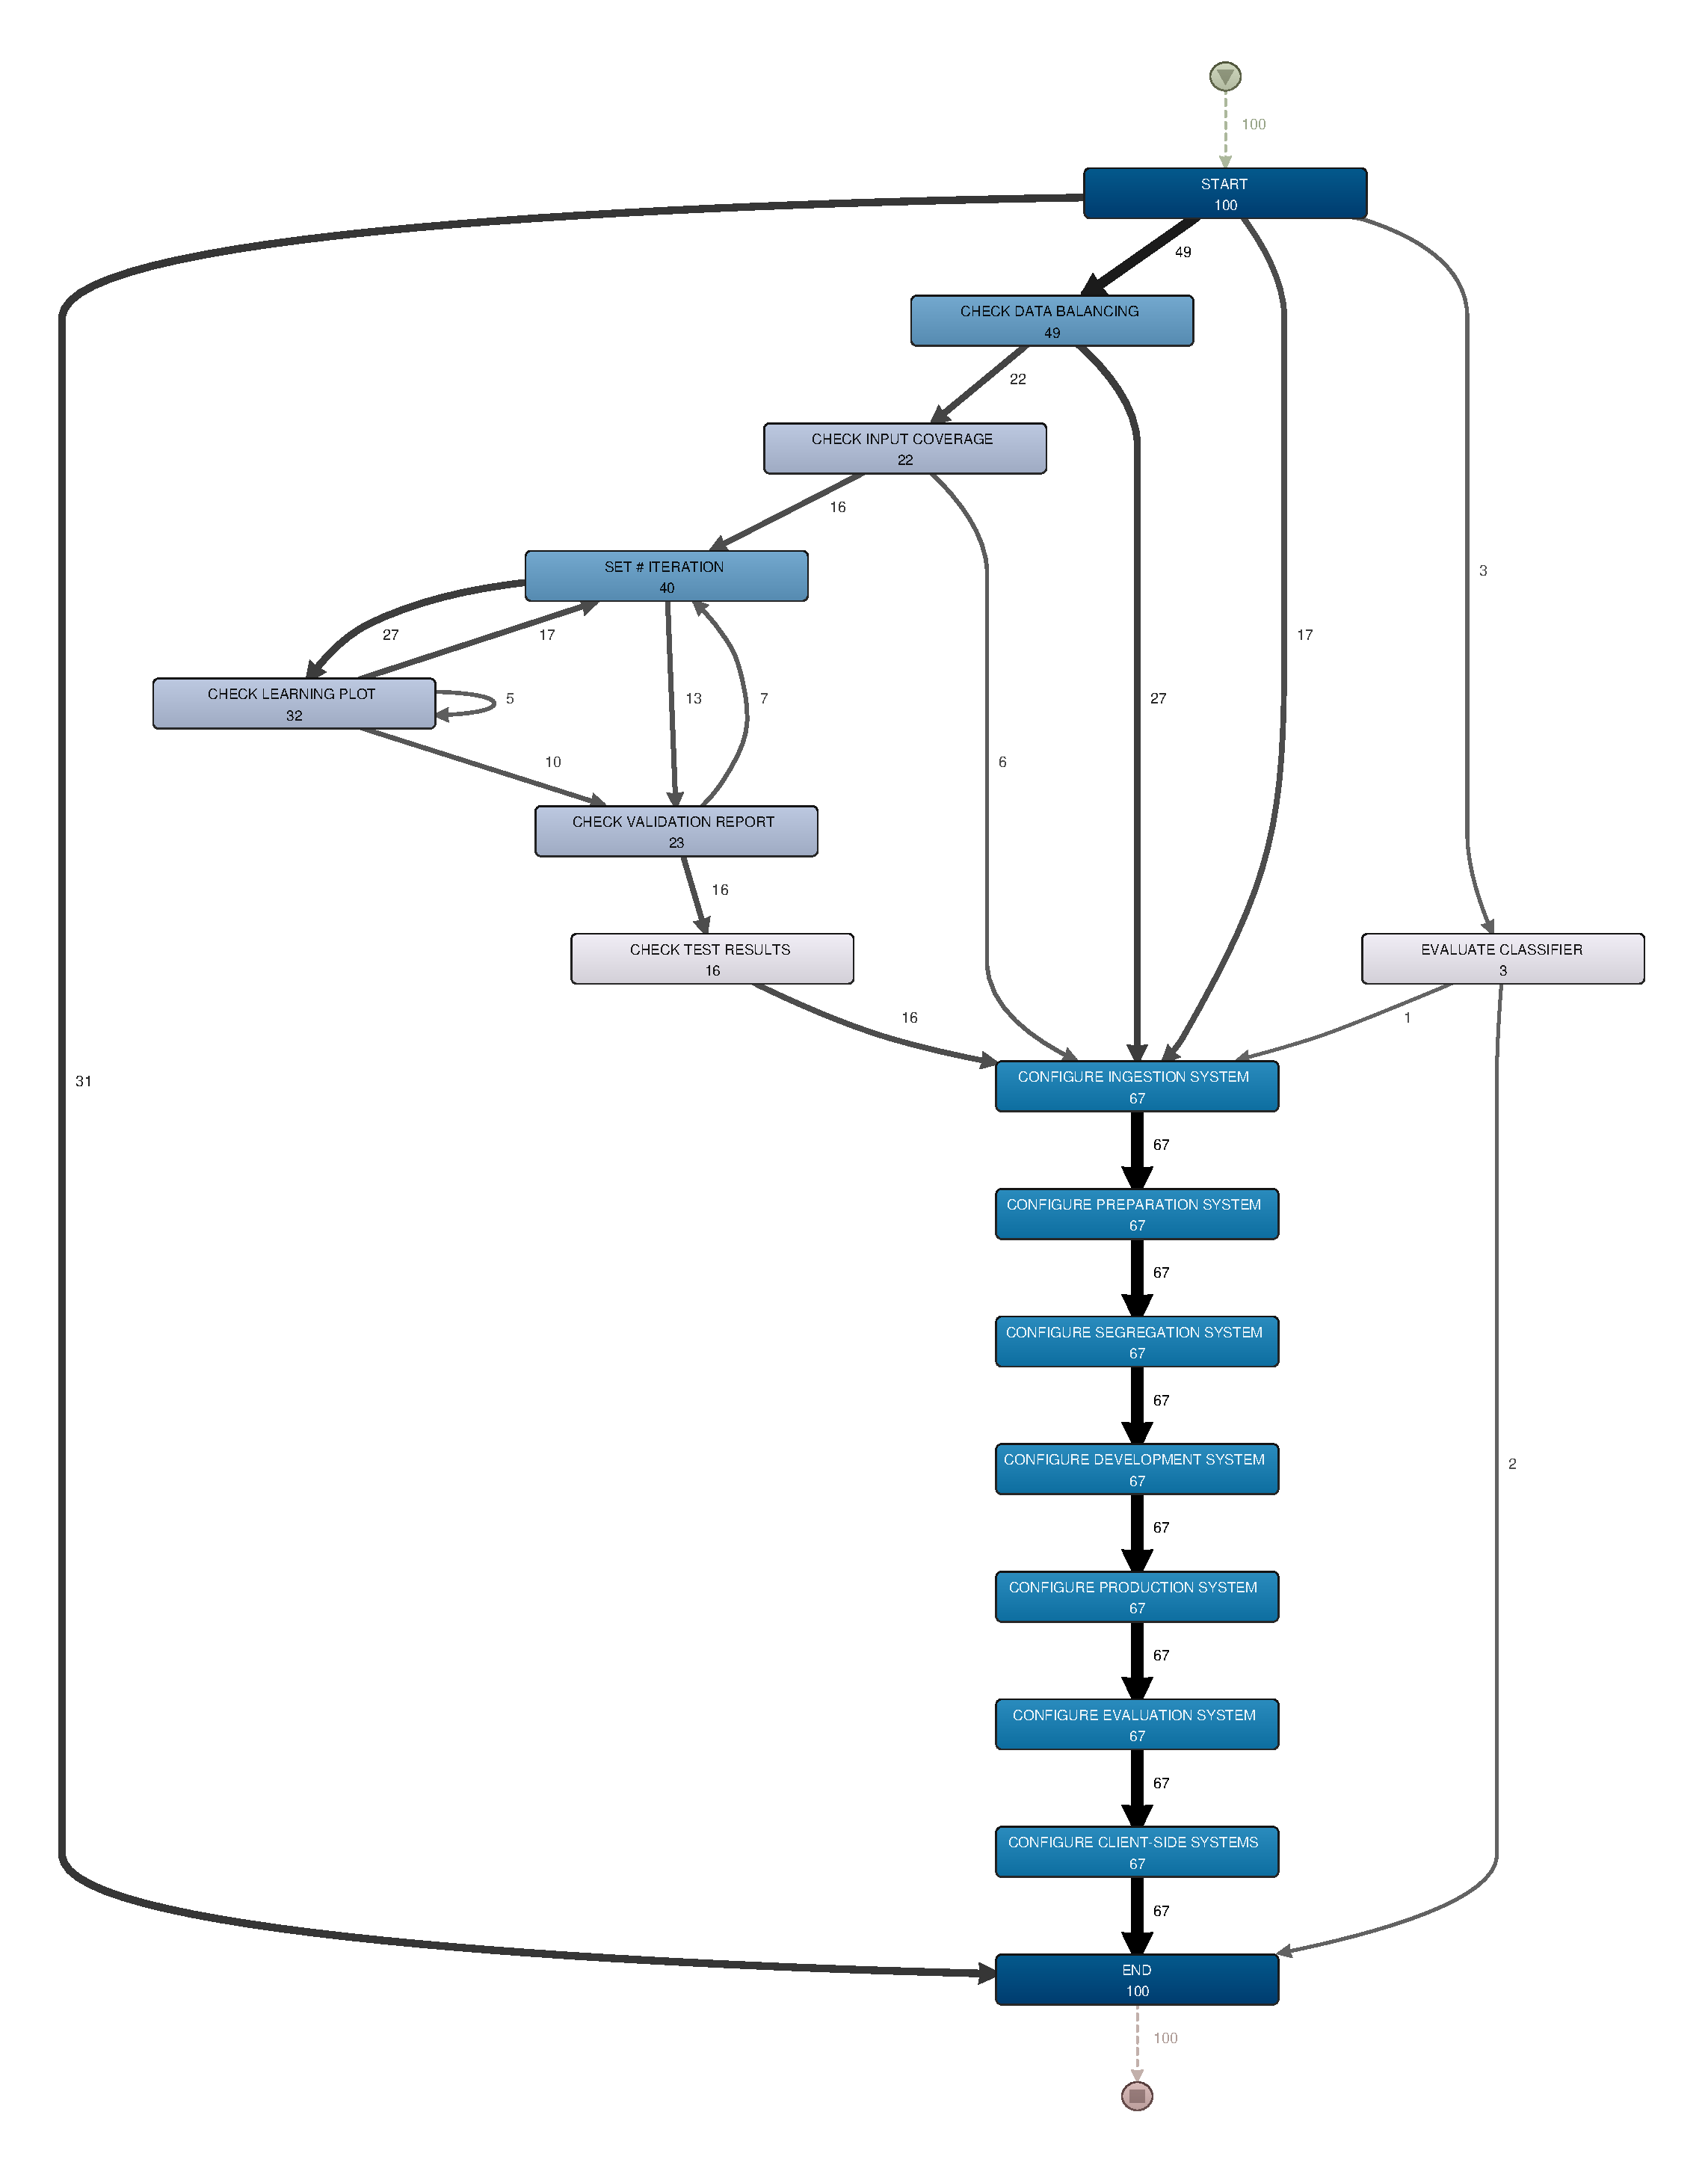
\includegraphics[width=0.8\textwidth]{figures/disco_map.pdf}
\caption{Disco analysis}
\label{fig:disco_analysis}
\end{figure}

\begin{figure}[H]
\centering
\includegraphics[width=\textwidth]{figures/apromore_map.pdf}
\caption{Apromore analysis}
\label{fig:apromore_analysis}
\end{figure}

As we can see, the two transition maps mined from Disco and from 
Apromore are identical.

\begin{figure}[H]
\centering
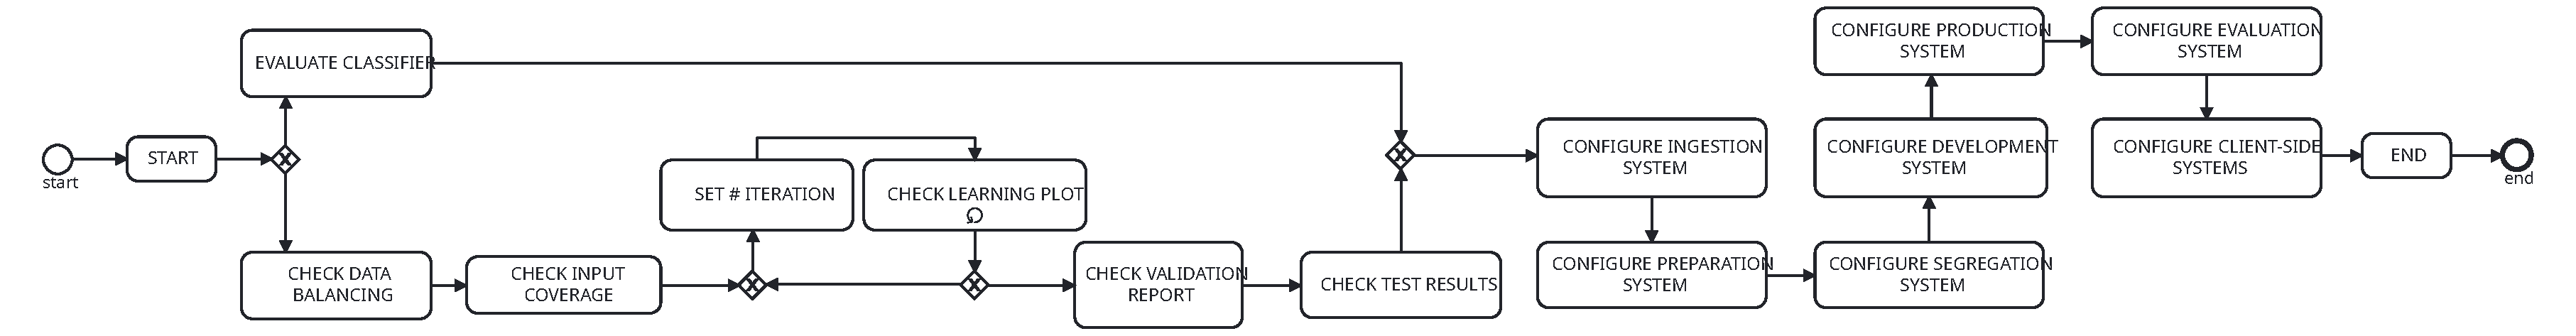
\includegraphics[width=\textwidth]{figures/prom_mined.pdf}
\caption{ProM mined BPMN model}
\label{fig:prom_mined}
\end{figure}

We mined the logs using the "Heuristics Miner ProM6" mining algorithm.

\begin{figure}[H]
\centering
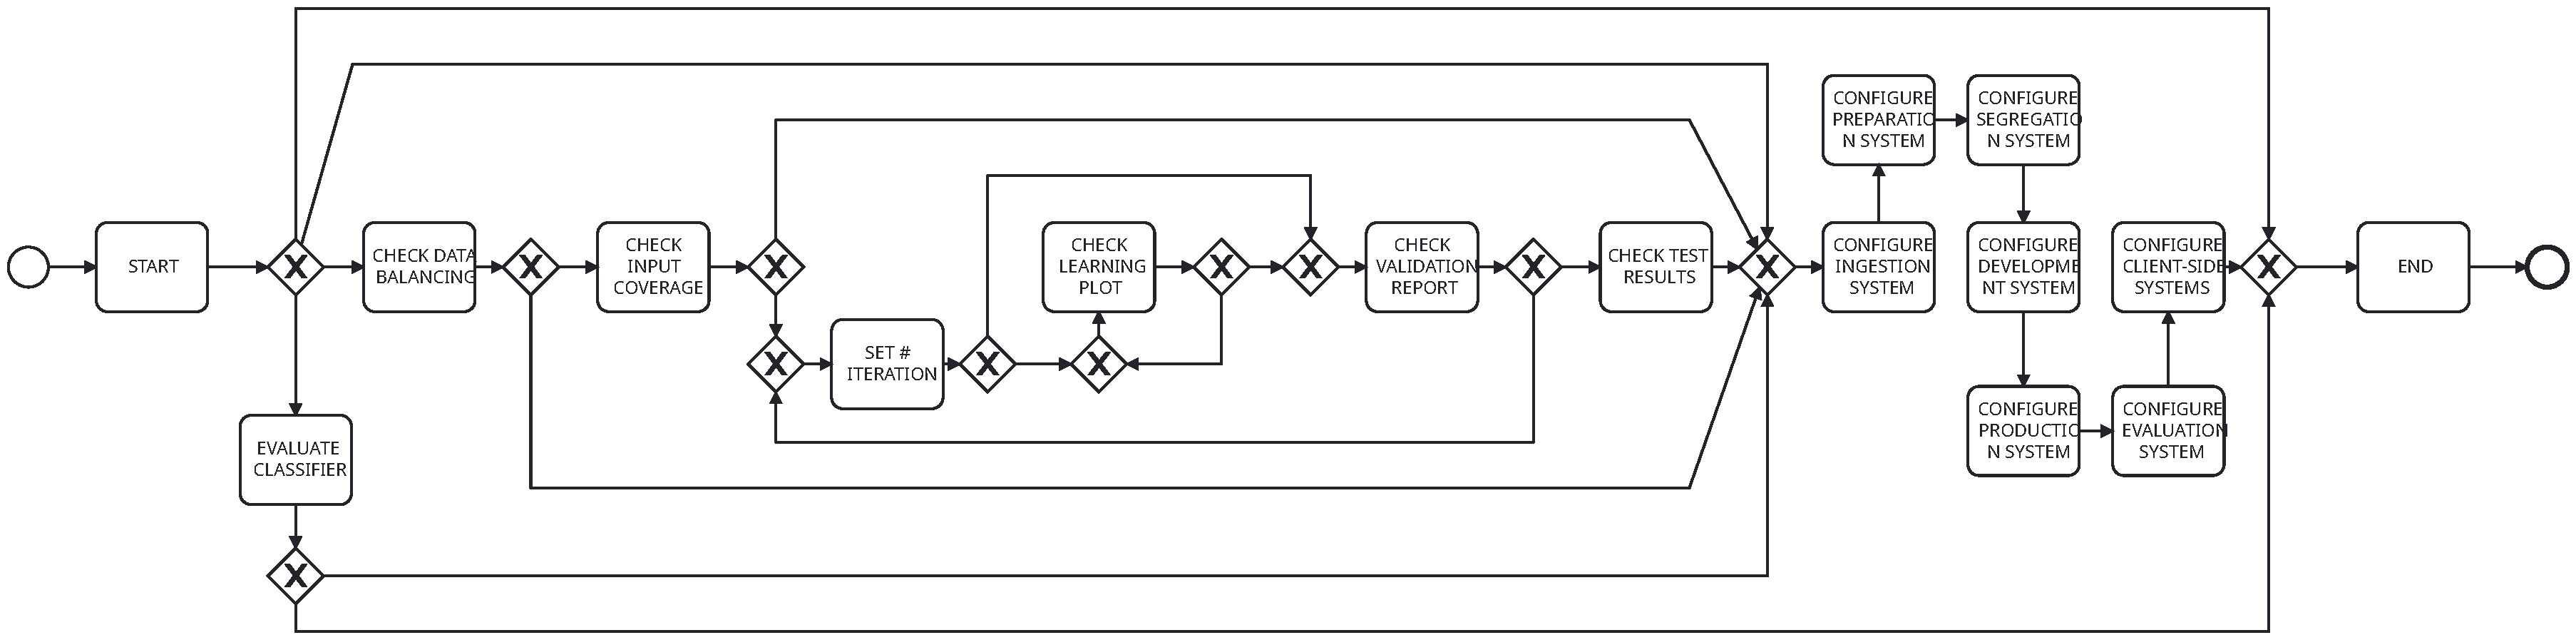
\includegraphics[width=\textwidth]{figures/apromore_mined.pdf}
\caption{Apromore mined BPMN model}
\label{fig:apromore_mined}
\end{figure}

The BPMN model mined from Apromore is more detailed and
covers more cases than the one mined from ProM.
Confronting the two models with the original BPMN, we can see that neither
of the two tools was able to recreate the training cycle accurately.

\begin{table}[H]
\centering
\begin{tabular}{|r|l|l|l|l|}
\hline
\textbf{Tool} & \textbf{Trace} & \textbf{Generalization} & \textbf{Precision} & \textbf{Simplicity} \\
\hline
Apromore & 0.4203 & 0.9872 & 0.7566 & 62 \\
\hline
ProM & 0.2917 & 0.9871 & 0.9871 & 39 \\
\hline
\end{tabular}
\caption{Comparison of the process mining tools}
\label{tab:process_mining_comparison}
\end{table}